
\documentclass{beamer}
\usecolortheme{dove}
\setbeamertemplate{navigation symbols}{}
\usepackage{amsmath,amssymb,amsfonts,amsthm, multicol, subfigure, color}
\usepackage{bm}
\usepackage{graphicx}
\usepackage{tabularx}
\usepackage{booktabs}
\usepackage{hyperref}
\usepackage{pdfpages}
\usepackage{xcolor}
\definecolor{seagreen}{RGB}{46, 139, 87}
\definecolor{mustard}{RGB}{234, 170, 0}
\def\independenT#1#2{\mathrel{\rlap{$#1#2$}\mkern2mu{#1#2}}}
\newcommand\indep{\protect\mathpalette{\protect\independenT}{\perp}}
\def\log{\text{log}}
\newcommand\logit{\text{logit}}
\newcommand\iid{\stackrel{\text{iid}}{\sim}}
\newcommand\E{\text{E}}
\newcommand\V{\text{V}}
\renewcommand\P{\text{P}}
\newcommand{\Cov}{\text{Cov}}
\newcommand{\Cor}{\text{Cor}}
\newcommand\doop{\texttt{do}}
\usepackage{stackrel}
\usepackage{tikz}
\usetikzlibrary{arrows,shapes.arrows,positioning,shapes,patterns,calc}
\newcommand\slideref[1]{\vskip .1cm \tiny \textcolor{gray}{{#1}}}
\newcommand\red[1]{\color{red}#1}
\newcommand\blue[1]{\color{blue}#1}
\newcommand\gray[1]{\color{gray}#1}
\newcommand\seagreen[1]{\color{seagreen}#1}
\newcommand\purple[1]{\color{purple}#1}
\newcommand\orange[1]{\color{orange}#1}
\newcommand\black[1]{\color{black}#1}
\newcommand\white[1]{\color{white}#1}
\newcommand\teal[1]{\color{teal}#1}
\newcommand\magenta[1]{\color{magenta}#1}
\newcommand\Fuchsia[1]{\color{Fuchsia}#1}
\newcommand\BlueGreen[1]{\color{BlueGreen}#1}
\newcommand\bblue[1]{\textcolor{blue}{\textbf{#1}}}
\newcommand\bred[1]{\textcolor{red}{\textbf{#1}}}
\newcommand\bgray[1]{\textcolor{gray}{\textbf{#1}}}
\newcommand\bgreen[1]{\textcolor{seagreen}{\textbf{#1}}}
\newcommand\bref[2]{\href{#1}{\color{blue}{#2}}}
\colorlet{lightgray}{gray!40}
\pgfdeclarelayer{bg}    % declare background layer for tikz
\pgfsetlayers{bg,main} % order layers for tikz
\newcommand\mycite[1]{\begin{scriptsize}\textcolor{darkgray}{(#1)}\end{scriptsize}}
\newcommand{\tcframe}{\frame{
%\small{
\only<1|handout:0>{\tableofcontents}
\only<2|handout:1>{\tableofcontents[currentsubsection]}}
%}
}

\newcommand{\goalsframe}{\begin{frame}{Learning goals for today}
By the end of class, you will be able to
\begin{itemize}
    \item conceptualize economic mobility in a machine learning framework
\end{itemize} \vskip .2in
\end{frame}}

\usepackage[round]{natbib}
\bibliographystyle{humannat-mod}
\setbeamertemplate{enumerate items}[default]
\usepackage{mathtools}

\title{Studying Social Inequality with Data Science}
\author{Ian Lundberg}
\date{\today}

\begin{document}

\begin{frame}
\begin{tikzpicture}[x = \textwidth, y = \textheight]
\node at (0,0) {};
\node at (1,1) {};
\node[anchor = north west, align = left, font = \huge] at (0,.9) {Studying\\Social Inequality\\with Data Science};
\node[anchor = north east, align = right] (number) at (1,.9) {INFO 3370 / 5371\\Spring 2023};
\node[anchor = north, font = \Large, align = right] at (.5,.5) {\bblue{Challenge: PSID Income Prediction}};
\end{tikzpicture}
\end{frame}

\goalsframe

\begin{frame}{Generalizing economic mobility}

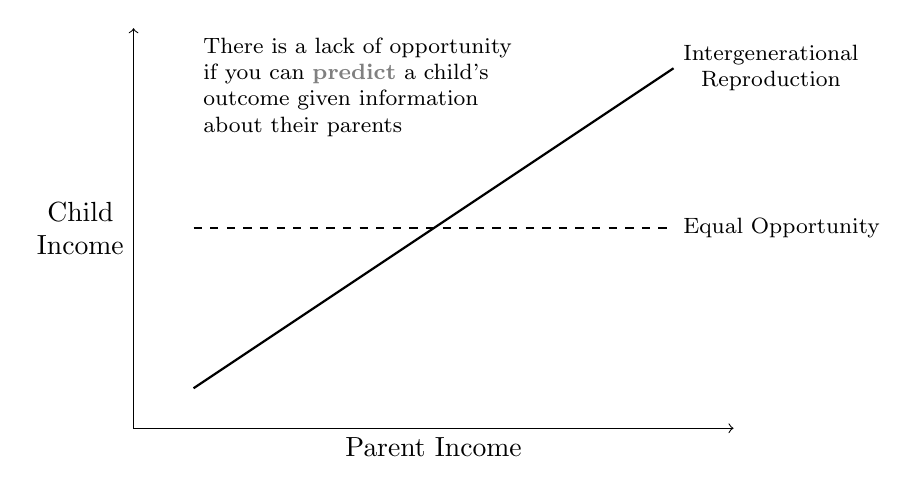
\begin{tikzpicture}[x = 3in, y = 2in]
\draw[<->] (1,0) -- (0,0) -- (0,1);
\node[anchor = east, align = center] at (0,.5) {Child\\Income};
\node[anchor = north, align = center] at (.5,0) {Parent Income}; \pause
\draw[thick, dashed] (.1,.5) -- (.9,.5);
\node[anchor = west, font = \footnotesize] at (.9,.5) {Equal Opportunity}; \pause
\draw[thick] (.1,.1) -- (.9,.9);
\node[anchor = west, font = \footnotesize, align = center] at (.9,.9) {Intergenerational\\Reproduction}; \pause
\node[anchor = north west, font = \footnotesize, align = left] at (.1,1) {There is a lack of opportunity\\if you can \bgray{predict} a child's\\outcome given information\\about their parents};
\end{tikzpicture}

\end{frame}

\begin{frame}

Why stop at parent income? \vskip .2in \pause
What other variables capture the luck of birth?

\end{frame}

\begin{frame}
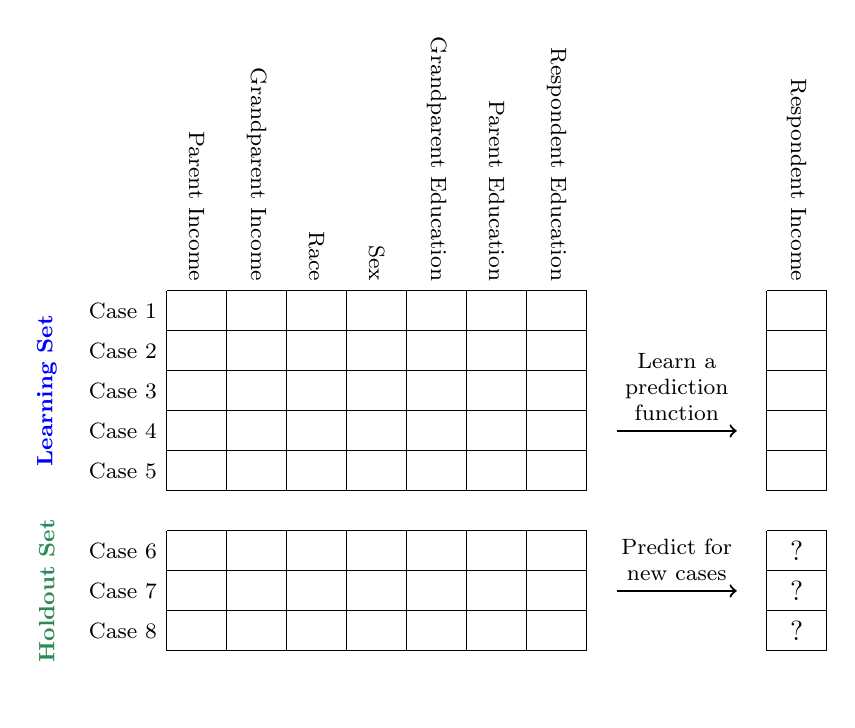
\begin{tikzpicture}[x = 3in, y = 2in]
\node[anchor = east, rotate = 270, font = \footnotesize] at (.15,1) {Parent Income};
\node[anchor = east, rotate = 270, font = \footnotesize] at (.25,1) {Grandparent Income};
\node[anchor = east, rotate = 270, font = \footnotesize] at (.35,1) {Race};
\node[anchor = east, rotate = 270, font = \footnotesize] at (.45,1) {Sex};
\node[anchor = east, rotate = 270, font = \footnotesize] at (.55,1) {Grandparent Education};
\node[anchor = east, rotate = 270, font = \footnotesize] at (.65,1) {Parent Education};
\node[anchor = east, rotate = 270, font = \footnotesize] at (.75,1) {Respondent Education};
\node[anchor = east, font = \footnotesize] at (.1,.95) {Case 1};
\node[anchor = east, font = \footnotesize] at (.1,.85) {Case 2};
\node[anchor = east, font = \footnotesize] at (.1,.75) {Case 3};
\node[anchor = east, font = \footnotesize] at (.1,.65) {Case 4};
\node[anchor = east, font = \footnotesize] at (.1,.55) {Case 5};
\draw[step=.1,black,thin] (0.1,.5) grid (.8,1); 
\node at (.5,1) {};
\pause
\node[anchor = east, rotate = 270, font = \footnotesize] at (1.15,1) {Respondent Income};
\draw[step=.1,black,thin] (1.1,.5) grid (1.2,1);
\draw[thin] (1.2,.5) -- (1.2,1);
\pause
\draw[->, thick] (.85,.65) -- node[midway, above, font = \footnotesize, align = center] {Learn a\\prediction\\function} (1.05,.65);
\pause
% Holdout set
\draw[step=.1,black,thin] (0.1,.1) grid (.8,.4);
\draw[step=.1,black,thin] (1.1,.1) grid (1.2,.4);
\draw[thin] (1.2,.1) -- (1.2,.4);
\node at (1.15,.35) {?};
\node at (1.15,.25) {?};
\node at (1.15,.15) {?};
\node[anchor = east, font = \footnotesize] at (.1,.35) {Case 6};
\node[anchor = east, font = \footnotesize] at (.1,.25) {Case 7};
\node[anchor = east, font = \footnotesize] at (.1,.15) {Case 8};
\pause
\draw[->, thick] (.85,.25) -- node[midway, above, font = \footnotesize, align = center] {Predict for\\new cases} (1.05,.25);
\pause
% Label the two
\node[rotate = 90, font = {\footnotesize\bf}, blue] at (-.1,.75) {{Learning} Set};
\node[rotate = 90, font = {\footnotesize\bf}, seagreen] at (-.1,.25) {{Holdout} Set};
\node at (-.05,0) {};
\end{tikzpicture}
\end{frame}

\begin{frame}{The challenge}
How well can you predict respondent incomes? \vskip .2in
Get started \bref{https://info3370.github.io/sp23/lessonplans/7b/}{here}
\end{frame}

\goalsframe

\end{document}

